\section{Introduction}

\subsection{The Art Gallery Problem \cite{o1987art}}

The Art Gallery Problem \cite{o1987art} is a central problem in computational geometry. It can be introduced as follows: given a simple polygon $\mathcal P$ with $n$ vertices, we are interested in finding the minimum number of guards (points) that are able to see the whole polygon. A simple polygon is a polygon that does not intersect itself when drawn in plane. Thus, we can define visibility in the polygon $\mathcal P \subset \mathbb R^2$ as a point (guard) $p \in \mathcal P$ being able to see another point $q \in \mathcal P$ if the line segment $\overline{pq} \subseteq \mathcal P$. The points that are visible from $p$ form the visibility polygon (region) $Vis(p)$. In the Art Gallery Problem, we are looking for a minimum size guard set $S$ that can see the whole polygon $\mathcal P$.

Figure \ref{fig:art} displays an example of The Art Gallery Problem \cite{o1987art} with polygon $\mathcal P$ guarded by 4 points ($|S| = 4$). The visibility region $\mathcal V$ of each guard is marked with a different colour. For point $p \in S$, its visibility region $Vis(p)$ is emphasised with the pink contour. In this case, the vertex $r$ blocks part of the view of $p$ and is called ``reflex'', because the angle it forms on the inside of the polygon is larger than $180^\circ$. Because reflex vertices are only found in concave polygons, convex polygons can be guarded by only one guard.

\begin{figure}[h!]
    \centering
    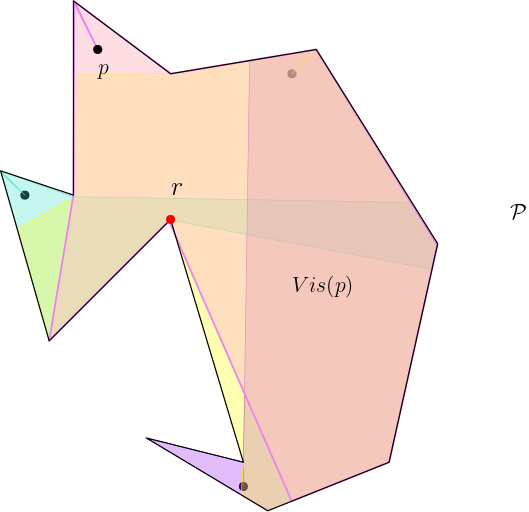
\includegraphics[width = 0.6\textwidth]{p.png}
    \caption{Example of an Art Gallery Problem instance with polygon $P$ guarded by 4 points. The visibility area $Vis(p)$ is highlit in pink.}
    \label{fig:art}
\end{figure}

The Art Gallery Problem \cite{o1987art} is $\exists \mathbb R$-complete \cite{abrahamsen2021art}, which means it does not accept solutions in polynomial space. For this reason, approximation algorithms have been extensively used to address it (\cite{DBLP:journals/corr/BonnetM16b}, \cite{GHOSH2010718}, \cite{DBLP:journals/corr/abs-2007-06920}). Nonetheless, there appeared to be no related work on approaching The Art Gallery Problem \cite{o1987art} using the gradient descent. As such, this paper will approach The Art Gallery Problem \cite{o1987art} from a new perspective using Gradient Descent.

\subsection{Gradient Descent}

Gradient descent is an iterative optimisation algorithm for finding the optimum of a continuous differentiable function. The idea of gradient descent is to repeatedly move in the opposite direction of the gradient of the function at the current point using a specific step size (speed). When there is no more change in the gradient, then the optimum has been reached. Gradient descent does not guarantee that the found optimum is global. For this reason, it can remain stuck in local optima.

\subsection{Thesis Goal}

The main goal of this thesis is to create and implement an algorithm that uses gradient descent to approximate the solution to The Art Gallery Problem \cite{o1987art} in reasonably fast time. The algorithm will be implemented in C ++ using the CGAL library (\url{https://www.cgal.org}). It will be then compared to other existing algorithm implementations.

As such, the initial research and work is presented as preparation for the thesis project. Chapter \ref{sec:literature} offers an existing literature overview. Next, Chapter \ref{sec:theory} describes the relevant theory in detail.
Lastly, Chapter \ref{sec:thesis} presents the development plan for the second phase of the Master's Thesis project.